\begin{table*}[t]
  \centering
  \begin{tabular}{@{}ccc@{}}
    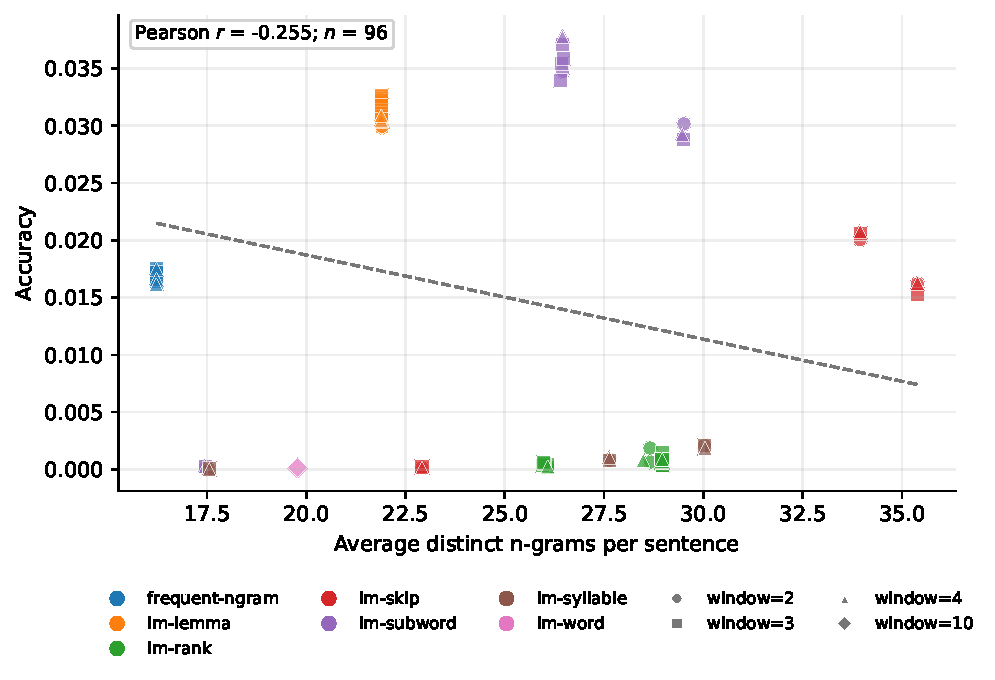
\includegraphics[
      width=0.315\textwidth,
      keepaspectratio
    ]{plots/avg-intrinsic.pdf}
    &
    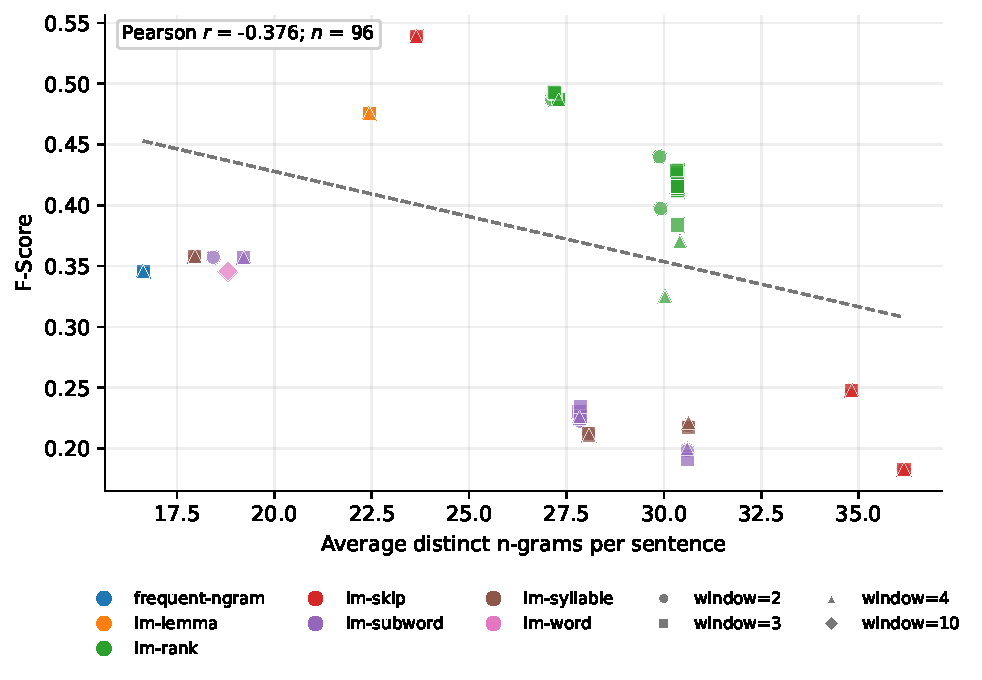
\includegraphics[
      width=0.315\textwidth,
      keepaspectratio
    ]{plots/avg-morphology.pdf}
    &
    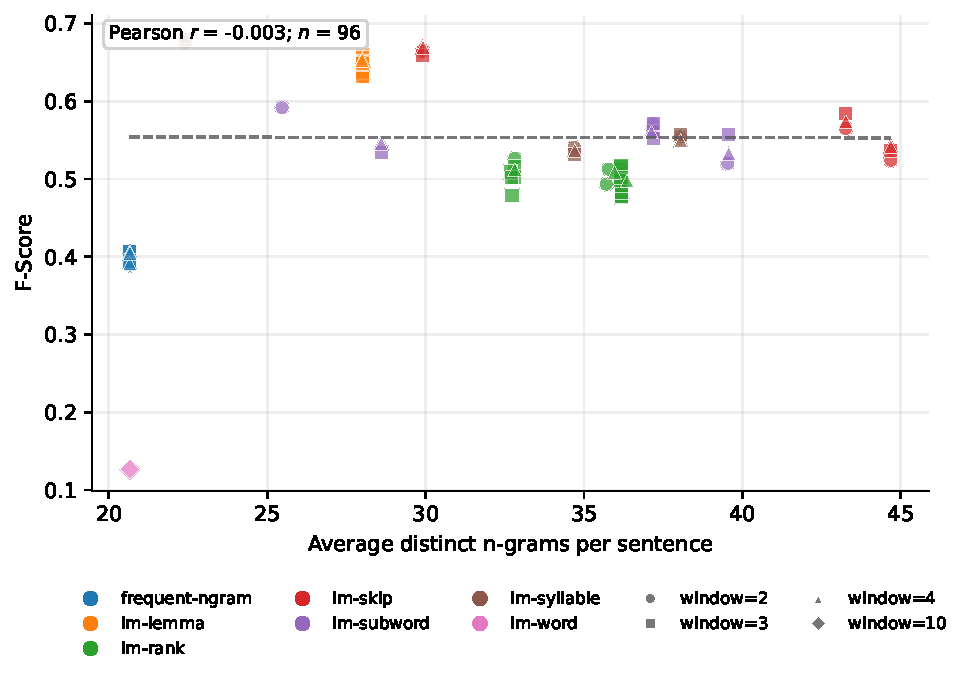
\includegraphics[
      width=0.315\textwidth,
      keepaspectratio
    ]{plots/avg-ner.pdf}
    \\
    Intrinsic & Morphology & NER
    \\
    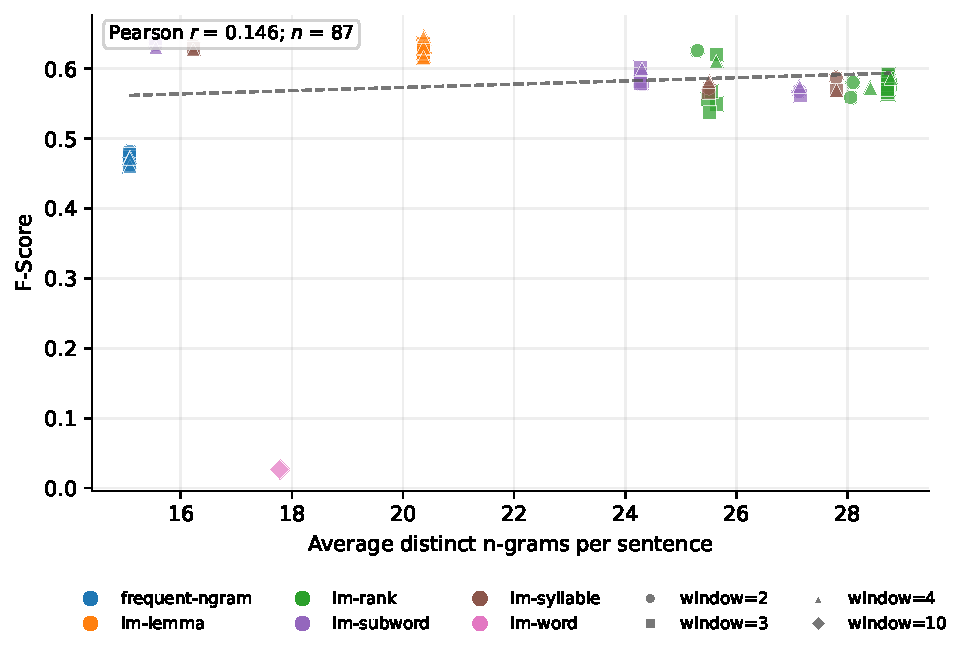
\includegraphics[
      width=0.315\textwidth,
      keepaspectratio
    ]{plots/avg-pos.pdf}
    &
    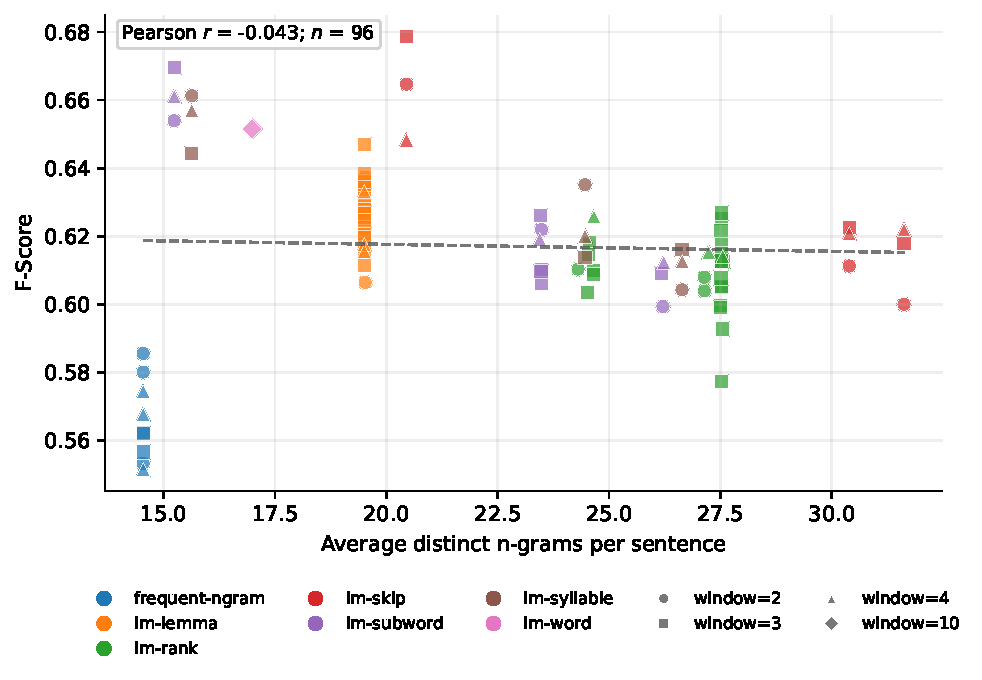
\includegraphics[
      width=0.315\textwidth,
      keepaspectratio
    ]{plots/avg-sentiment.pdf}
    &
    {}
    \\
    POS & Sentiment & {}
  \end{tabular}
  \caption{Average number of distinct LM n-grams per sentence and task
  performance. Intrinsic uses Accuracy; Morphology, NER, POS, and Sentiment
  use F-measure.}
  \label{tab:avg}
\end{table*}

\subsection{Distinct n-gram diversity and task performance}

Table~\ref{tab:avg} examines whether the average number of distinct LM
n-grams in a sentence is associated with downstream performance. For each
stored partition corpus, the number of unique partitions is first calculated
within every sampled sentence and then averaged over at most 10,000 non-empty
sentences. This statistic measures local representational diversity: larger
values indicate that a typical sentence contains a wider variety of
partition units. Intrinsic performance is represented by Accuracy, while
Morphology, NER, POS, and Sentiment are represented by F-measure.

No consistent relationship emerges across tasks. The descriptive Pearson
correlation is negative for Intrinsic Accuracy ($r=-0.255$) and the
Morphology reference estimate ($r=-0.376$). NER ($r=-0.003$) and Sentiment
($r=-0.043$) are approximately uncorrelated with distinct-n-gram diversity,
whereas POS shows a weak positive association ($r=0.146$). Thus, increasing
the number of distinct partitions in a sentence does not uniformly improve
or degrade performance. The result suggests that the linguistic relevance
and selection of the partitions are more consequential than their quantity
alone.

As in the density analysis, these correlations combine variation in LM
method, window length, and other partition parameters and therefore do not
identify an independent causal effect. All NER rows are current; the POS panel
excludes the nine legacy rows without Precision and Recall. Morphology
requires an additional limitation: its direct evaluator does not save a
partitioned corpus, so its x-axis value is the mean distinct-n-gram count of
the same LM variant across the four stored partition corpora. A future
evaluation should save the Morphology partitions and repeat the analysis
using a directly measured, task-specific value.
